\documentclass[12pt]{article}
\usepackage[spanish,mexico]{babel}
	\selectlanguage{spanish}
\usepackage{graphicx}
\usepackage{amsmath}
\usepackage{wrapfig}
\usepackage{float}
\usepackage{hyperref}
\usepackage[utf8]{inputenc}


\title{Actividad 4: Ajuste de datos con mínimos cuadrados}
\author{Ana Gabriela Carretas Talamante}
\date{12 de febrero de 2016}

\begin{document}
\maketitle
\section{Introducción}
En el área de la estadística, hay un campo denominado análisis de regresión cuya misión es poder obtener modelos matemáticos, como las funciones, para diversos comportamientos de fenómenos observados. Tras tener una colección de datos, estos se analizan y con diferentes métodos, se llega a facilitar el estudio del fenómeno con funciones conocidas, como las rectas, parábolas o exponenciales.

Mínimos cuadrados es una técnica de análisis numérico enmarcada dentro de la optimización matemática, en la que, dados un conjunto de pares ordenados: variable independiente, variable dependiente, y una familia de funciones, se intenta encontrar la función continua, dentro de dicha familia, que mejor se aproxime a los datos (un ``mejor ajuste''), de acuerdo con el criterio de mínimo error cuadrático \cite{W}. 

\begin{figure}[H]
\centering
\includegraphics[width=6cm]{0}
\caption{Ejemplo de una regresión lineal con una variable dependiente y una variable independiente \cite{L}.}
\end{figure}

La técnica de los mínimos cuadrados es parte de ambas secciones en el análisis de la regresión, pues se puede utilizar tanto en la regresión lineal como en el no lineal. En la actividad de hoy, se utilizaron ambos métodos para poder ajustar funciones del tipo lineal y exponencial a dos conjuntos de datos distintos con una herramienta que nos proporciona el paquete Scipy de Python.

El método \textit{scipy.optimze.leastsq} encuentra el conjunto de parámetros que minimizan la función de error. Este comienza a partir de una primera conjetura y trata de minimizar la función de error cada que entran los datos proporcionados, y así devuelve la lista de los parámetros que mejor se ajusten a los datos \cite{Q}. 

En los programas presentados a continuación, se leen los datos obtenidos de los siguientes sitios, donde se registraron las \href{http://www.seattlecentral.edu/qelp/sets/048/048.html}{temperaturas medias de invierno en Nueva York} y la \href{http://www.seattlecentral.edu/qelp/sets/024/024.html}{presión atmosférica con respecto a al altura}. Se utilizaron los paquetes especificados de \textit{Scipy}: \textit{curve\_fit; leastsq}.

\subparagraph*{Programa 1: Ajuste lineal}
Se denomina regresión lineal cuando la función es lineal, es decir, requiere la determinación de dos parámetros: la pendiente y la ordenada en el origen de la recta de regresión, $y=ax+b$. La regresión nos permite además, determinar el grado de dependencia de las series de valores $X$ e $Y$, prediciendo el valor $y$ estimado que se obtendría para un valor $x$ que no esté en la distribución \cite{RL}. \\

Se presenta a continuación el código ajustando linealmente los datos de la temperatura media en los inviernos de 1900-1999 en Nueva York.

\begin{verbatim}
import numpy as np
import matplotlib.pyplot as plt
from scipy import optimize

#Leyendo el archivo con los datos
datos = np.loadtxt('lineal.txt')
x=datos[:,0]
y=datos[:,1]

print x
print y

#Escribiendo con la forma de y=mx+b
fitfunc = lambda p, x: p[0]*x + p[1]

#Distancia del punto al ajuste lineal
errfunc = lambda p, x, y: fitfunc(p, x) - y 

#Parametros patito
p0 = [1, 1] 

#Optimizando la recta
p1, success = optimize.leastsq(errfunc, p0[:], args=(x, y))

#Para la grafica
time = np.linspace(x.min(), x.max(), 100)
plt.plot(x, y, "mo", label="Data") 
plt.plot(time, fitfunc(p1, time), "g-", label="Fitted curve")

plt.title("Winter temperature in New York from 1900-1999")
plt.grid()
plt.legend()
plt.xlabel("Year")
plt.ylabel("Temperature")
\end{verbatim}

\begin{figure}[H]
\centering
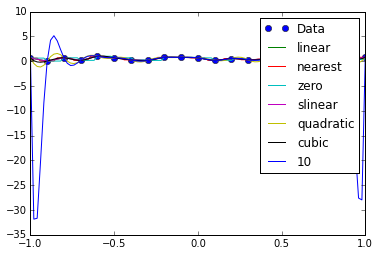
\includegraphics[width=9cm]{1}
\caption{Gráfica generada por el programa.}
\end{figure}

\subparagraph*{Programa 2: Ajuste exponencial}
Será aquella en la que la función de ajuste será una función exponencial del tipo $y = ab^x$ \cite{RE}. La regresión exponencial, aunque no es lineal, es linealizable tomando logaritmos ya que haciendo el cambio de variable $v=log y$ tendremos que la función anterior nos generaría: $$v=log y=log( ab^x)=log a + x log b $$

Se presenta a continuación el código ajustando exponencialmente los datos de la presión atmosférica (mb) en función de la altura (km).

\begin{verbatim}
import numpy as np
import matplotlib.pyplot as plt
from scipy.optimize import curve_fit

#Leyendo el archivo con los datos
datos = np.loadtxt('exponencial.txt')
x=datos[:,0]
y=datos[:,1]
print x
print y

#Escribiendo con la forma de y=a*e^(-bx)+c
def func(x, a, b, c):
    return a * np.exp(-b * x) + c

#Generando estimacion base
yn = y + 0.2*np.random.normal(size=len(x))

#Optimizando la curva
popt, pcov = curve_fit(func, x, yn)

#Para la grafica
plt.figure()
plt.plot(x, yn, 'mo', label="Data")
plt.plot(x, func(x, *popt), 'g-', label="Fitted curve")

plt.grid()
plt.legend()
plt.title("Atmospheric pressure vs. altitude")
plt.xlabel("Altitude")
plt.ylabel("Pressure")

plt.show()
\end{verbatim}

\begin{figure}[H]
\centering
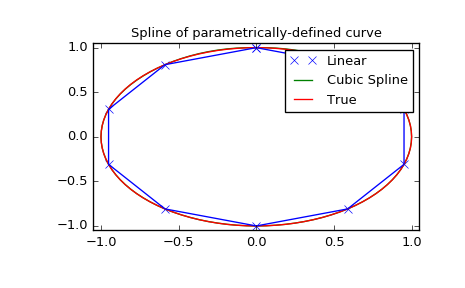
\includegraphics[width=9cm]{2}
\caption{Gráfica generada por el programa.}
\end{figure}

\pagebreak

\begin{thebibliography}{6}

\bibitem{W}
Wikipedia,
\emph{Mínimos cuadrados}. Recuperado el 12 de febrero de 2016 de \url{https://es.wikipedia.org/wiki/M\%C3\%ADnimos_cuadrados}

\bibitem{L}
Wikipedia,
\emph{Linear regression}. Recuperado el 12 de febrero de 2016 de \url{https://es.wikipedia.org/wiki/Regresi\%C3\%B3n_lineal\#/media/File:Linear_regression.svg}

\bibitem{Q}
Qiku programación,
\emph{Cómo utilizar leastsq función desde scipy.optimize en python para adaptarse tanto a una línea recta y una línea cuadrática para conjuntos de datos x e y}. Recuperado el 12 de febrero de 2016 de \url{http://goo.gl/giZ7rO}

\bibitem{RL}
\emph{Regresión lineal}. Recuperado el 12 de febrero de 2016 de \url{http://www.sc.ehu.es/sbweb/fisica/cursoJava/numerico/regresion/regresion.htm}

\bibitem{RE}
\emph{Regresión exponencial}. Recuperado el 12 de febrero de 2016 de \url{https://www.uv.es/ceaces/base/regresion/exponenci.htm}

\bibitem{E}
IanVS,
\emph{Ajuste exponencial y logarítmico}. Recuperado el 12 de febrero de 2016 de 
\url{http://goo.gl/j6Ottu}

\bibitem{S1}
Scipy,
\emph{leastsq}. \url{http://docs.scipy.org/doc/scipy/reference/generated/scipy.optimize.leastsq.html#scipy.optimize.leastsq}

\bibitem{S2}
Scipy,
\emph{curve\_fit}. \url{http://docs.scipy.org/doc/scipy/reference/generated/scipy.optimize.curve_fit.html}

\bibitem{FC}
Lizárraga, C.
\emph{Actividad 3 (2016-1)}. Recuperado el 12 de febrero de 2016 de \url{http://computacional1.pbworks.com/w/page/105016164/Actividad\%204\%20(2016-1)}

\end{thebibliography}

\end{document}